\documentclass{article}
\usepackage{parskip}
\usepackage{caption}
\usepackage{fancyhdr}
\usepackage{amsmath}
\usepackage{lastpage} 
\usepackage{hyperref}
\usepackage{graphicx} % Required for inserting images
\usepackage[margin=0.9in,top=1in,includefoot]{geometry}
\usepackage{framed} % or, "mdframed"
\usepackage[framed]{ntheorem}
\usepackage{theoremref}
\newframedtheorem{frm-thm}{Theorem}
\makeatletter
\newcommand*{\toccontents}{\@starttoc{toc}}
\newcommand{\ans}{\subsection*{Løsning}}
\makeatother


\newcommand{\RR}{\mathbb{R}}
\newcommand{\NN}{\mathbb{N}}
\newtheorem{thm}{Conjecture}

\setcounter{section}{1}

\begin{document}


\author{Ask Madsen}
\title{Løsning til mindstekravsopgaverne}
\maketitle

\toccontents
\newpage


\subsubsection{Opgave 1}

Nedenfor er et udtryk reduceret.\\
\begin{align*}
    4&\cdot (5a-b)+b-3a\\
    &=20a-4b+b-3a\\
    &=17a-3b
\end{align*}
Forklar hvert trin i reduktionen\\\\

\subsubsection*{Løsning opgave 1}
I det første trin ganger vi 4 ind i parentesen på hvert led således
\begin{align*}
    4\cdot (5a-b)=4\cdot 5a - 4\cdot b=20a-4b
\end{align*}

I det næste trin samler vi ledene som indeholder a og ledene som indeholder b således
\begin{align*}
    20a -4b + b - 3a = 20a - 3a - 4b + b = 17a - 3b
\end{align*}

\newpage
\subsection{Opgave 2}

Nedenfor er en ligning løst.
\begin{align*}
    3x + 2(x+1) + 7 &= 5\\
    3x + 2x + 2 + 7 &= 5\\
    5x + 9 &= 5\\
    5x &= -4\\
    x &= -\frac{4}{5}
\end{align*}
Forklar, hvad der er gjort i hvert trin.\\\\

\ans
I det første trin ganger vi 2 tallet ind i parentesen på hvert led således 
\begin{align*}
    2(x + 1)=2x + 2
\end{align*}
I det næste trin lægger vi ledene som indeholder x sammen og ledene som ikke indeholder x sammen.
\begin{align*}
    3x + 2x +2 +7 = 5x + 9
\end{align*}
I det næste trin trækker vi 9 fra på begge sider
\begin{align*}
    5x + 9 - 9 = 5 - 9 \Longleftrightarrow 5x = -4
\end{align*}
I det sidste trin dividerer vi med 5 
\begin{align*}
    \frac{5x}{5} = -\frac{4}{5} \Longleftrightarrow x = -\frac{4}{5}
\end{align*}

\newpage
\subsection{Opgave 3}

Forklar, at værdien af $a^2 - (b+c)$ er 1, når $a = -3$, $b = 6$ og $c = 2$.\\\\

\ans
Vi starter med at indsætte værdierne for a, b og c hvorefter vi beregner parentesen og potensen og trækker så resultaterne fra hinanden
\begin{align*}
    (-3)^2 - (6 + 2) = 9 - 8 = 1
\end{align*}


\newpage
\subsubsection{Opgave 4}

Hvor mange procent udgør 30 ud af 260?\\\\

\subsubsection*{Løsning opgave 4}
For at bestemme hvor mange procent Tal1 udgør af Tal2 kan man bruge følgende formel
\begin{align*}
    \frac{Tal1}{Tal2}\cdot 100\%
\end{align*}
Hvis vi indsætter de kendte værdier Tal1$=30$ og Tal2$=260$ får vi
\begin{align*}
    \frac{30}{260}\cdot 100 \approx 11.53 \%
\end{align*}
30 udgør altså ca 11.53 \% af 260.
\vspace*{1cm}
\newpage
\subsubsection{Opgave 5}

Løs følgende to ligninger med to ubekendte
\begin{align*}
   &x = 6 - y\\
    &5y + x = 14
\end{align*}

\subsubsection*{Løsning opgave 5}

Vi indsætter den første ligning $x = 6-y$ på x's plads i den anden ligning således
\begin{align*}
    5y + (6 - y) = 14
\end{align*}
I denne ligning isolerer vi så y
\begin{align*}
    &5y + (6 - y) = 14\\
    \Updownarrow \; &\\
    &5y - y + 6 = 14\\
    \Updownarrow \; &\\
    &4y + 6 = 14\\
    \Updownarrow \; &\\
    &4y = 14 - 6\\
    \Updownarrow \; &\\
    &4y = 8\\
    \Updownarrow \; &\\
    &\frac{4y}{4} = \frac{8}{4}\\
    \Updownarrow \; &\\
    &y = 2
\end{align*}
Indsætter nu $y = 2$ i den første ligning og får
\begin{align*}
    x = 6 - 2 = 4
\end{align*}
Løsningen til de 2 ligninger er derfor $x = 4$ og $y = 2$. 
\newpage
\subsubsection{Opgave 6}

Bestem diskriminanten for andengradsligningen
\begin{align*}
    3x^2 + 4x -1 = 0
\end{align*}

\subsubsection*{Løsning opgave 6}

Den generelle formel for diskriminanten er $d = b^2 - 4\cdot a\cdot c$. Vi ved at den generelle andengradsligning skrives på formen $ax^2 + bx + c = 0$. Vi aflæser nu a, b og c og får følgende $a = 3,\; b = 4,\; c = -1$. Diskriminanten bliver dermed
\begin{align*}
    d = 4^2 -4\cdot 3\cdot (-1) = 16 - (-12) = 16 + 12 = 28
\end{align*}
\newpage
\subsubsection*{Opgave 7}

Løs denne ligning: $\cfrac{20}{x+2} = 4$\\\\

\subsubsection*{Løsning opgave 7}
Vi starter med at dividere med 20 på begge sider
\begin{align*}
    \frac{20}{20(x+2)}=\frac{4}{20} \Longrightarrow \frac{1}{x+2} = \frac{4}{20}
\end{align*}
Nu kan vi bytte om på tæller og nævner på begge sider af lighedstegne så vi får
\begin{align*}
    x+2 = \frac{20}{4}
\end{align*}
Nu trækker vi 2 fra på begge sider og får
\begin{align*}
    x + 2 - 2 = \frac{20}{4}- 2
\end{align*}
Ved at omskrive 2 tallet til $2 = \frac{8}{4}$ får vi nu
\begin{align*}
    x = \frac{20}{4}-\frac{8}{4}=\frac{20-8}{4}=\frac{12}{4}=3
\end{align*}
\newpage
\subsubsection{Opgave 8}

Undersøg om $x = 2$ er en løsning til denne ligning: $x^2 -5x + 6 = 0$.\\\\

\subsubsection*{Løsning opgave 8}

For at undersøge om $x = 2$ er en løsning til ligningen indsætter vi 2 på x's plads og ser om venstresiden giver 0.
\begin{align*}
    2^2 -5\cdot 2 + 6 = 4 - 10 + 6 = 10 - 10 = 0
\end{align*}
$x = 2$ er altså en løsning til ligningen. 
\newpage
\subsection{Opgave 9}

To linjer er givet ved $y = 4x -1$ og $y = x  + 5$. Bestem skæringspunktet mellem de to linjer.\\\\


\ans
For at bestemme skæringspunktets x-koordinat mellem de to linjer kan vi sætte dem lig med hinanden og isolere for x.
\begin{align*}
    &4x -1 = x + 5\\
    \Updownarrow \; &\\
    &4x -1 + 1 = x + 5 + 1\\
    \Updownarrow \; &\\
    &4x = x + 6\\
    \Updownarrow \; &\\
    &4x - x = x - x + 6\\
    \Updownarrow \; &\\
    &3x = 6\\
    \Updownarrow \; &\\
    &\frac{3x}{3} = \frac{6}{3}\\
    \Updownarrow \; &\\
    &x = 2
\end{align*}
Herefter indsætter vi $x = 2$ i en af de to linjers forskrift og bestemmer skæringspunktets y-koordinat
\begin{align*}
    y = 2 + 5 = 7
\end{align*}
Skæringspunktet mellem de to linjer er derfor $(2,7)$
\newpage
\subsection{Opgave 10}

Isolér $T$ i ligningen $a\cdot T = \frac{R-T}{Q+a}$.\\\\

\ans
Vi starter med at gange med $(Q+a)$ på begge sider
\begin{align*}
    a\cdot T \cdot (Q+a) = \frac{R-T}{Q+a}\cdot (Q+a) \Longrightarrow aQT + a^2T = R-T
\end{align*}
Vi lægger nu $T$ til på begge sider
\begin{align*}
    aQT + a^2T + T = R 
\end{align*}
Nu sætter vi $T$ uden for en parentes så $(aQ + a^2 + 1)T = aQT + a^2T + T$
\begin{align*}
    (aQ + a^2 + 1)T = R
\end{align*}
Dividerer nu med $(aQ + a^2 + 1)$ på begge sider og får
\begin{align*}
    T = \frac{R}{aQ + a^2 + 1}
\end{align*}
$T$ er hermed isoleret i ligningen.


\subsection{Opgave 11}
Figuren viser en trekant $ABC$.\\\\
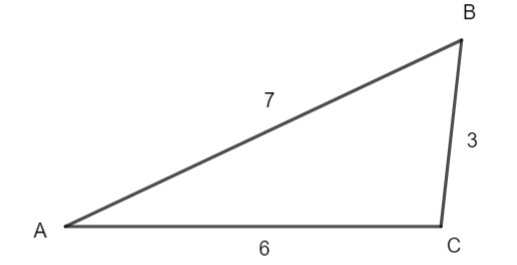
\includegraphics[width=10cm]{Opgave_11-20/Opgave_11/Opgave_11.jpg}

Følgende sidelængder er kendte: $|AB| = 7,\; |BC| = 3$ og  $|AC| = 6$.\\\\
Bestem vinkel $A$.\\\\


\ans
Da trekanten ikke er retvinkel kan vi bruge cosinusrelationen
\begin{align*}
    a^2 = b^2 + c^2 -2\cdot b\cdot c\cdot \cos(A)
\end{align*}
Her isolerer vi først cos(A)
\begin{align*}
    &a^2 -b^2 - c^2 = -2\cdot b\cdot c\cdot \cos(A)\\
    \Updownarrow \; &\\
    &\frac{a^2 - b^2 - c^2}{-2\cdot b\cdot c} = \cos(A)\\
    \Updownarrow \; &\\
    &-\frac{a^2 - b^2 - c^2}{2\cdot b\cdot c} = \cos(A)
\end{align*}
Nu indsætter vi sidelængderne på a,b og c's plads så $a = 3,\; b = 6$ og $c = 7$
\begin{align*}
    &-\frac{3^2 - 6^2 - 7^2}{2\cdot 6\cdot 7} = \cos(A)\\
    \Updownarrow \; &\\
    &-\frac{9 - 36 - 49}{84} = \cos(A)\\
    \Updownarrow \; &\\
    &-\frac{-76}{84} =  \cos(A)\\
    \Updownarrow \; &\\
    &\frac{76}{84} = \cos(A)\\
\end{align*}
Nu bruger vi den inverse funktion til cos altså arccos for at bestemme vinklen A
\begin{align*}
    A = \arccos\left(\frac{76}{84}\right) \approx 25.2 ^{\circ}
\end{align*}
\newpage
\subsection{Opgave 12}
To ensvinklede trekanter er vist på figuren.\\\\
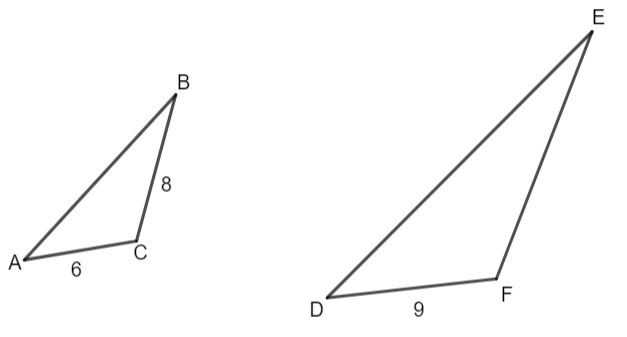
\includegraphics[width=10cm]{Opgave_11-20/Opgave_12/Opgave_12.jpg}\\\\
\textbf{Størrelsesforholdene er ikke korrekte.}\\\\

Følgende sidelængder oplyses: $|AC| = 6,\; |BC| = 8$ og $|DF| = 9$\\\\

Bestem $FE|$\\\\

\ans
Da trekanterne er ensvinklede kan vi altså bestemme sidelængdernes størrelsesforhold. Hvis vi ser på sidelængderne $|AC|$ og $|DF|$ er den større trekants side 1.5 gange længere. Vi kan altså bestemme sidelængden $|FE| = 1.5\cdot |BC| = 1.5\cdot 8 = 12$. 
\newpage
\subsection{Opgave 13}

Figuren viser en trekant\\\\
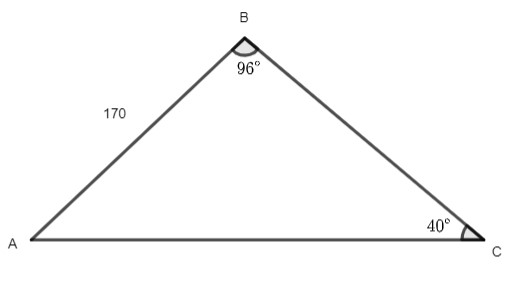
\includegraphics[width=10cm]{Opgave_11-20/Opgave_13/Opgave_13.jpg}\\\\
Følgende størrelser i trekant $ABC$ er kendte:\\\\
$B = 96^{\circ},\quad |AB| = 170\quad \text{og}\quad C = 40^{\circ}$\\\\

Bestem $|AC|$.\\\\

\ans
For at bestemme længden af siden $AC$ bruger vi sinusrelationen for en vilkårlig trekant
\begin{align*}
    \frac{a}{\sin(A)} = \frac{b}{\sin(B)} = \frac{c}{\sin(C)}
\end{align*}
Her svarer sidelængen $AB$ til c og sidelængden $AC$ som vi skal finde svarer til b. Vi betragter den sidste lighed i sinusrelationen og isolerer b.
\begin{align*}
    \frac{b}{\sin(B)} =\frac{c}{\sin(C)} \Longleftrightarrow b = \frac{c}{\sin(C)}\cdot \sin(B)
\end{align*}
Indsætter nu $c = 170,\quad C = 40^{\circ},\quad B = 96^{\circ}$ og får 
\begin{align*}
    b = \frac{170}{\sin(40^{\circ})}\cdot \sin(96^{\circ})\approx 263.03
\end{align*}
\newpage
\subsection{Opgave 14}

En retvinklet trekant er skitseret på figuren.\\\\
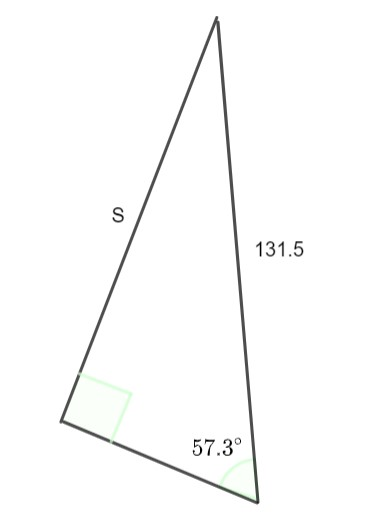
\includegraphics[width=7cm]{Opgave_11-20/Opgave_14/Opgave_14.jpg}\\\\
Bestem længden S.\\\\

\ans
For retvinklede trekanter gælder formlen
\begin{align*}
    \sin(B) = \frac{c}{b}
\end{align*}
Her er B vinklen $B = 57.3^{\circ}$, c er længden af hypotinusen dvd $c = 131.5$ og b er siden som i vores tilfælde svarer til s. Vi isolerer altså b og indsætter tallene
\begin{align*}
    \sin(B) = \frac{b}{c} \Longleftrightarrow b = \sin(B)\cdot c = \sin(57.3^{\circ})\cdot 131.5 \approx 89.76
\end{align*}

\newpage
\subsection{Opgave 15}

Et punkt har koordinatsættet $A(8,6)$.\\\\
En linje $l$ har ligningen $y = -x+7$.\\\\
Bestem afstanden mellem $A$ og $l$.\\\\

\ans
Her bruger vi formlen for afstand mellem et punkt og en linje som siger at afstanden fra et punkt $(x_1,y_1)$ til en linje $y = ax+b$ kan bestemmes ved
\begin{align*}
    \text{dist}(P,m)=\frac{|ax_1+b-y_1|}{\sqrt{a^2 +1}}
\end{align*}
Vi indsætter tallene og får
\begin{align*}
    \text{dist}(P,m)=\frac{|(-1)\cdot 8+7-6|}{\sqrt{(-1)^2 + 1}}= \frac{|-8+1|}{\sqrt{1+1}}=\frac{|-7|}{\sqrt{2}}=\frac{7}{\sqrt{2}}\approx 4.95
\end{align*}
\newpage
\subsection{Opgave 16}

En cirkel $C$ og en linje $l$ er bestemt ved ligningerne
\begin{align*}
    C&:(x-4)^2 + (y-5)^2 = 3^2\\
    l&:y = x-2
\end{align*}
 a) Tegn cirklen og linjen i samme koordinatsystem.\\

 \ans
 Vi starter med at aflæse cirklens centrumskoordinat og cirklens radius. Vi ved at cirklens generelle ligning er givet ved
 \begin{align*}
     (x-a)^2 + (y-b)^2 = r^2
 \end{align*}
 Her er $C(a,b)$ cirklens centrumskoordinat og r er cirklens radius. Hvis vi bruger dette kan vi aflæse centrumskoordinatet til $C(4,5)$ og radius til $r = 3$. Vi kan nu indtegne cirklen i et koordinatsystem\\\\
 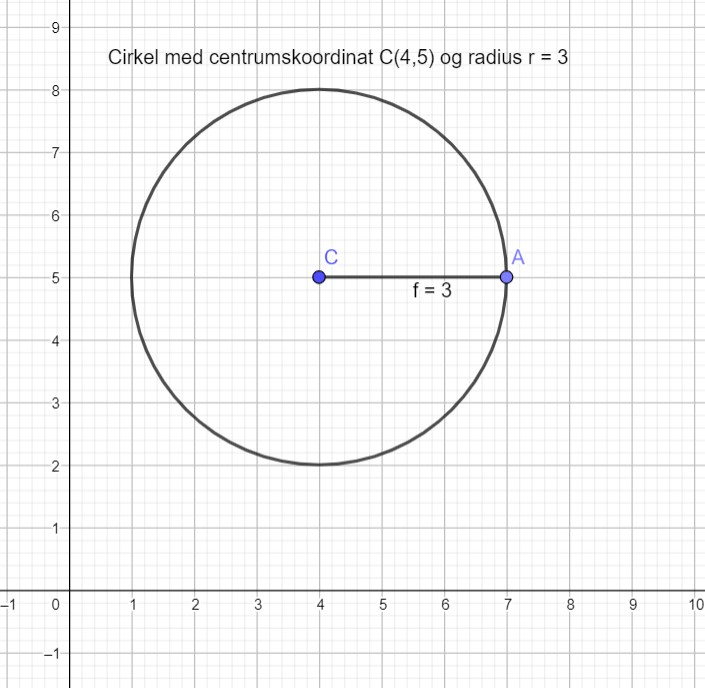
\includegraphics[width=8cm]{Opgave_11-20/Opgave_16/16.jpg}\\\\
 
 For at indtegne linjen skal vi aflæse linjens hældning, a og linjens skærings med y-aksen, b. Vi ved at en ret linje har den generelle form
 \begin{align*}
     y = ax+b
 \end{align*}
 Aflæser vi nu den givne linje får vi hældningen $a = 1$ og skæringen med y-aksen $b = -2$. Ud fra disse oplysninger kan vi nu indtegne vores linje i koordinatsystemet\\\\
 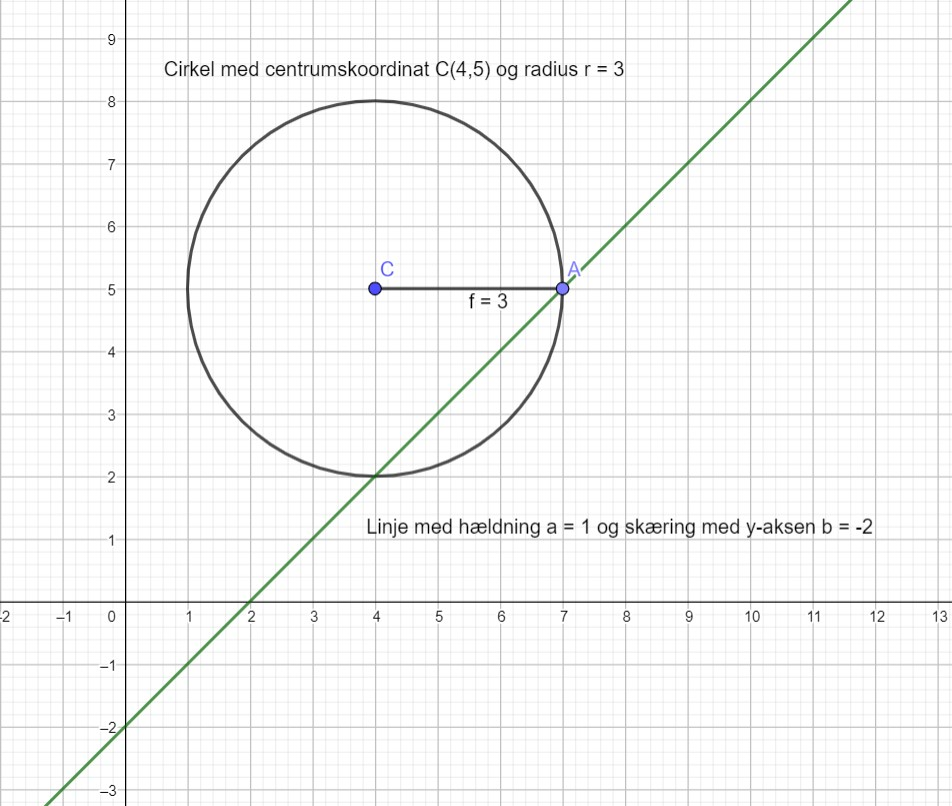
\includegraphics[width = 8cm]{Opgave_11-20/Opgave_16/16.1.jpg}\\\\
 
 b) Bestem skæringspunkterne mellem cirklen og linjen\\\\

 \ans
 
 Ud fra koordinatsystemet i opgave 16a kan vi se at cirklen og linjen skærer hinanden i 2 punkter. For at bestemme disse skæringspunkter sætter vi linjens ligning $y = x-2$ ind på y's plads i cirklens ligning
 \begin{align*}
     &(x-4)^2 + (x-2-5)^2 = 3^2\\
     \; \Updownarrow &\\
     &(x-4)^2 + (x-7)^2 = 9\\
 \end{align*}
 Vi beregner nu de 2 parenteser ved at bruge reglen $(a-b)^2 = a^2+2\cdot a\cdot (-b) + (-b)^2$
 \begin{align*}
     (x-4)^2 = x^2 +2\cdot x \cdot (-4) + (-4)^2 = x^2 -8x + 16\\
     (x-7)^2 = x^2 +2\cdot x \cdot (-7) + (-7)^2 = x^2 -14x + 49
 \end{align*}
 Indsætter vi dette får vi nu
 \begin{align*}
    &(x-4)^2 + (x-7)^2 = 9\\
    \; \Updownarrow &\\ 
    &x^2-8x+16+x^2-14x+49 = 9\\
    \; \Updownarrow &\\
    &x^2+x^2 -8x - 14x + 16+49=9\\
    \; \Updownarrow &\\
    &2x^2 - 22x + 65 = 9
 \end{align*}
 Vi trækker nu 9 fra på begge sider 
 \begin{align*}
     &2x^2 -22x +65-9 = 9-9\\
     \; \Updownarrow &\\
     &2x^2 -22x 56 = 0
 \end{align*}
 Nu findes vi løsningerne til det ovenstående andengradsligning ved først at beregne determinanten 
 \begin{align*}
     d = b^2 -4ac = (-22)^2 -4\cdot 2\cdot 56 = 36
 \end{align*}
 Nu bestemmer vi løsningerne altså x-koordinatet til skæringen mellem cirklen og linjen
 \begin{align*}
     x_1 = \frac{-b+\sqrt{d}}{2a}=\frac{22+\sqrt{36}}{2\cdot 2}=\frac{22+6}{4}=\frac{28}{4}=7\\
     x_2 = \frac{-b-\sqrt{d}}{2a}=\frac{22-\sqrt{36}}{2\cdot 2}=\frac{22-6}{4}=\frac{16}{4} = 4
 \end{align*}
 For at finde de tilsvarende skæringer med y-aksen indsætter vi de fundne x-værdier i linjens ligning
 \begin{align*}
     y_1 = x_1 -2 = 7-2 = 5\\
     y-2 = x_2 -2 = 4-2 = 2
 \end{align*}
 Vi har altså føgende skæringspunkter mellem linjen og cirklen
 \begin{align*}
     S_1=(x_1, y_1)=(7,5)\\
     S_2 =(x_2,y_2)=(4,2)
 \end{align*}
 Hvis vi sammenligner med tegningen vi får fra opgave 16a kan vi se at skærngspunkterne stemmer.
\newpage
\subsection{Opgave 17}

En cirkel $C$ er givet ved ligningen
\begin{align*}
    C:(x-2)^2 + (y-3)^2 = 5^2
\end{align*}
Bestem cirklens centrum og radius\\\\

\ans

Hvis vi benytter os af den generelle formel for cirklens ligning fra opgave 16 kan vi aflæse cirklens centrum til $C(2,3)$ og cirklens radius til $r = 5$

\newpage
\subsection{Opgave 18}

Undersøg om punktet $(2,3)$ ligger på linjen bestemt ved $2x + y - 7 = 0$\\\\

\ans
For at tjekke om et punkt ligger på en bestemt linje indsætter vi punktets x-koordinat på x'plads og punktets y-koordinat på y's plads.
\begin{align*}
    2\cdot 2 + 3 - 7 = 4 + 3 -7 = 7-7 =0
\end{align*}

Da venstresiden af vores beregning stemmer med højresiden altså 0 kan vi konkludere at punktet $(2,3)$ ligger på linjen.
\newpage
\subsection{Opgave 19}

På figuren ses en linje i et koordinatsystem.\\\\
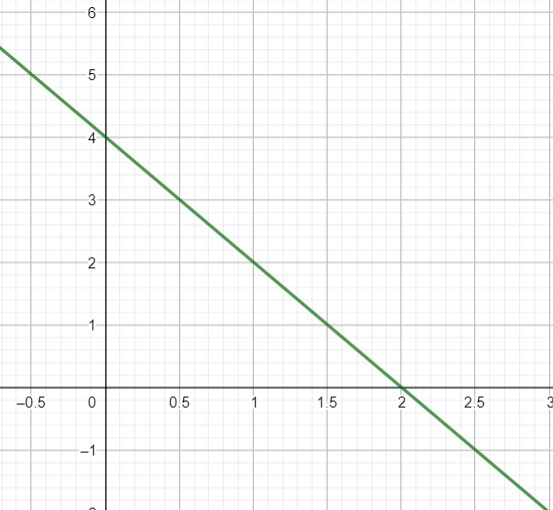
\includegraphics[width=8cm]{Opgave_11-20/Opgave_19/19.jpg}\\\\
Bestem en ligning for linjen.\\\\

\ans
Vi ved at en linje som denne har den generelle form $y = ax + b$. Her er a hældningen og b er skæringen med y-aksen. Vi aflæser skæringen med y-aksen på grafen til $b = 4$. For at bestemme hældningen $a$ skal vi benytte os af følgende formel
\begin{align*}
    a = \frac{y_2-y_1}{x_2-x_1}
\end{align*}
Her er $(x_1,y_1)$ og $(x_2,y_2)$ to vilkårlige punkter på vores linje. For nemhedens skyld vælger vi punkterne til at være 
\begin{align*}
    (x_1,y_1) = (0,4)\\
    (x_2,y_2) = (2,0)
\end{align*}
Indsætter vi disse punkter i formlen bestemmer vi nu a
\begin{align*}
    a = \frac{0-4}{2-0}=\frac{-4}{2}=-2
\end{align*}
Linjens ligning er derfor
\begin{align*}
    y = -2x + 4
\end{align*}
\newpage
\subsection{Opgave 20}

En vektor $\Vec{a}$ er bestemt ved
\begin{align*}
    \Vec{a} = \begin{pmatrix}-1 \\ 4\end{pmatrix}
\end{align*}
Indtegn vektoren i et koordinatsystem, og bestem $|\Vec{a}|$\\\\

\ans
Hvis vi lader vores vektor starte i punktet (0,0) så fortæller vektorens koordinater os at vi skal bevæge os -1 hen ad x-aksen og 4 op ad y-aksen. Forbinder vi disse punkter og tegner en pil op for enden af stregen får vi følgende graf\\\\
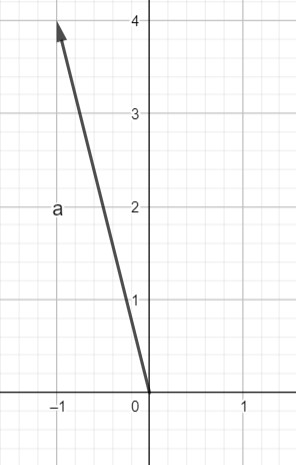
\includegraphics[width = 6cm]{Opgave_11-20/Opgave_20/20.jpg}
\newpage


\subsection{Opgave 21}

To vektorer $\Vec{a}$ og $\Vec{b}$ er givet ved
\begin{align*}
    \Vec{a} = \begin{pmatrix}-3 \\ 4\end{pmatrix}\; \text{og}\; \Vec{b} = \begin{pmatrix}1 \\ 3\end{pmatrix}
\end{align*}
Bestem vektor $\Vec{c}$, når $\Vec{c} = \Vec{a}+2\Vec{b}$\\\\

\ans
Vi kan bestemme vektor c bed følgende
\begin{align*}
    \Vec{c} = \Vec{a} + 2\Vec{b} = \begin{pmatrix}-3 \\ 4\end{pmatrix} + 2\begin{pmatrix}1 \\ 3\end{pmatrix}=\begin{pmatrix}-3 \\ 4\end{pmatrix} + \begin{pmatrix}2\cdot 1 \\ 2\cdot 3\end{pmatrix}=\begin{pmatrix}-3 \\ 4\end{pmatrix} + \begin{pmatrix}2 \\ 6\end{pmatrix}=\begin{pmatrix}-3+2 \\ 4+6\end{pmatrix} = \begin{pmatrix}-1 \\ 10 \end{pmatrix} 
\end{align*}
\newpage
\subsection{Opgave 22}

En vektor $\Vec{a}$ er bestemt ved
\begin{align*}
    \Vec{a} = \begin{pmatrix}5\cdot \cos(60^{\circ}) \\ 5\cdot \sin(60^{\circ})\end{pmatrix}
\end{align*}
Forklar hvad tallene 5 og $60^{\circ}$ fortæller om $\Vec{a}$\\\\

\ans
Tallet 5 fortæller os at $\Vec{a}$ har længden 5. Tallet $60^{\circ}$ er vektorens retningsvinkel altså den vinkel der er mellem vektoren og x-aksen. Dette kan ses illustreret på følgende graf\\\\
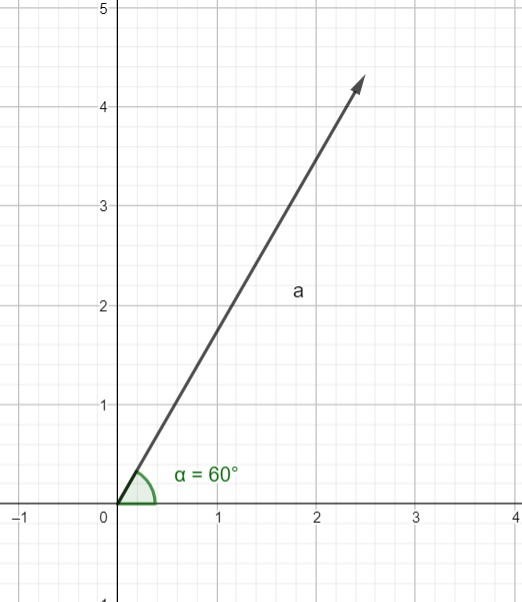
\includegraphics[width = 6cm]{Opgave_21-30/Opgave_22/22.jpg}
\newpage
\subsection{Opgave 23}

En vektor $\Vec{c}$ har længden 6 og retningsvinklen $127^{\circ}$\\\\
Bestem koordinaterne for $\Vec{c}$.\\\\

\ans
For at bestemme vektor c's koordinaterne gør vi bruge af følgende formel
\begin{align*}
    \Vec{c} = \begin{pmatrix}l\cdot \cos(v) \\ l\cdot \sin(v)\end{pmatrix}
\end{align*}
Her er l vektorens længde og v er vektorens retningsvinkel. Indsætter vi de givne værdier får vi
\begin{align*}
    \Vec{c} = \begin{pmatrix}6\cdot \cos(127^{\circ}) \\ 6\cdot \sin(127^{\circ})\end{pmatrix} = \begin{pmatrix}-3.61 \\ 4.79\end{pmatrix}
\end{align*}
Vektoren er illustreret nedenfor\\\\
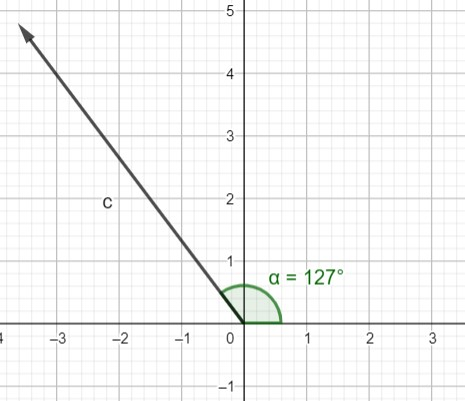
\includegraphics[width = 6cm]{Opgave_21-30/Opgave_23/23.jpg}
\newpage
\subsection{Opgave 24}

På figuren nedenfor ses repræsentanter for vektorerne $\vec{a}$, $\vec{b}$ og $\vec{c}$.

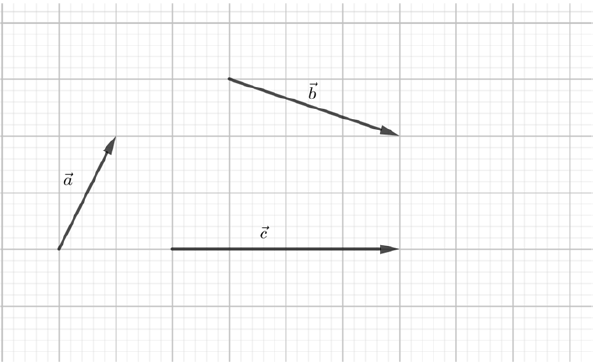
\includegraphics[width = 0.5\textwidth]{Opgave_21-30/Opgave_24/24.png}

Indtegn en repræsentant for vektoren $\vec{a} + \vec{b} + \vec{c}$.

\ans

Først aflæser vi vektorernes x og y komponenter. X komponenten af en vektor er hvor meget vi går hen ad x - aksen, og y komponent er hvor meget vi går op ad y aksen. Nedenstående figur illustrerer hvordan man kan aflæse en vektors x og y komponenter ud fra figuren. 

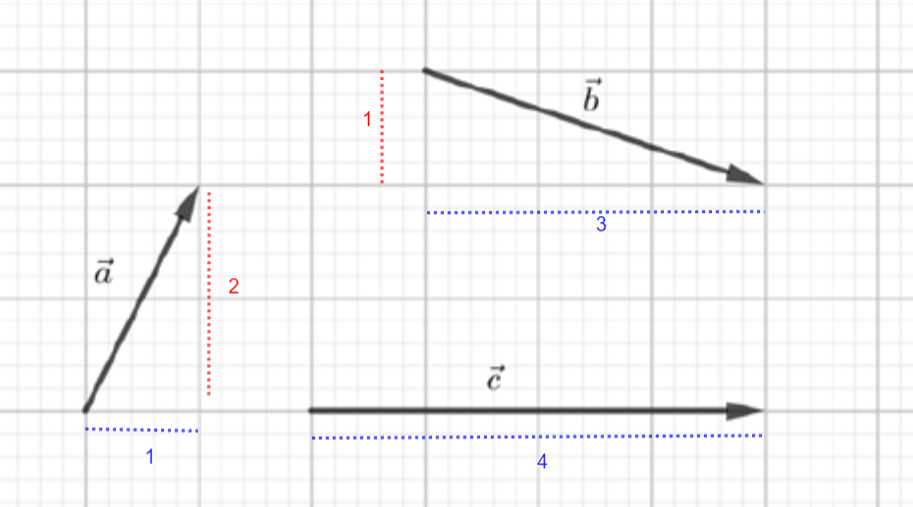
\includegraphics[width = 0.5\textwidth]{Opgave_21-30/Opgave_24/24.1.png}

De blå linjer er vektorernes x komponenter og de røde linjer er vektorernes y komponenter.

Vi har nu
\begin{align*}
    \Vec{a} &= \begin{pmatrix} 1 \\ 2 \end{pmatrix}\\
    \Vec{b} &= \begin{pmatrix} 3 \\ -1 \end{pmatrix}\\
    \Vec{c} &= \begin{pmatrix} 4 \\ 0 \end{pmatrix}
\end{align*}

Vi kan nu beregne summen af de 3 vektorer
\begin{align*}
    \Vec{a} + \Vec{b} + \Vec{c} = \begin{pmatrix} 1 \\ 2 \end{pmatrix} + \begin{pmatrix} 3 \\ -1 \end{pmatrix} + \begin{pmatrix} 4 \\ 0 \end{pmatrix} = \begin{pmatrix}
        1 + 3 + 4 \\ 2 - 1 + 0
    \end{pmatrix}  = \begin{pmatrix}
        8 \\ 1
    \end{pmatrix}
\end{align*}

Nu indtegner vi vektoren $\begin{pmatrix}
    8 \\ 1
\end{pmatrix}$
ind i et koordinatsystem. 

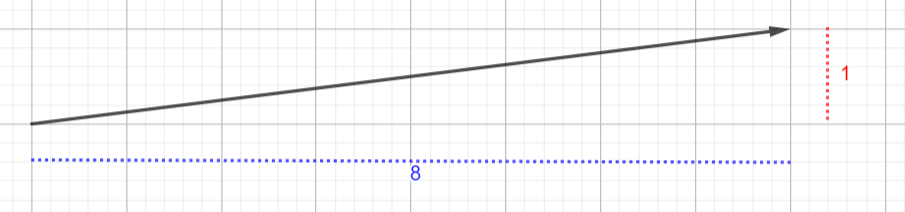
\includegraphics[width = 0.5\textwidth]{Opgave_21-30/Opgave_24/24.2.png}
\newpage
\subsection{Opgave 25}

På figuren nedenfor ses grafen for en funktion f.

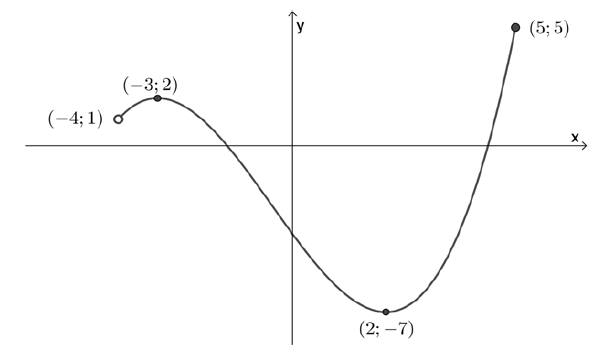
\includegraphics[width=10cm]{Opgave_21-30/Opgave_25/25.png}

Benyt figuren til at bestemme definitionsmængden og værdimængden for funktionen.

\ans

Definitionsmængden for en funktion f (Dm(f)) er alle de tilladte x værdier som funktionen kan have.
Kigger vi på figuren og går langs x-aksen støder vi først på punktet (-4;1). Den laveste x værdi funktionen f kan tage er derfor -4.
Det sidste punkt vi støder på er punktet (5,5). Den højeste x værdi funktionen f kan tage er dermed 5.


Vi opskriver nu definitionsmængden for funktionen f som intervallet mellem dens laveste og højeste x værdi.
Da det første punkt (-4; 1) var åbent hører den laveste x værdi ikke med og den første parentes er derfor åben (vender derfor udad) $\rbrack$.
Da det sidste punkt (5; 5) bar lukket hører den højeste x værdi med og den sidste parentes er derfor lukket (vender indad) $\rbrack$.
Vi får definitionsmængden

\begin{align*}
    Dm(f) = \rbrack-4; 5\rbrack
\end{align*}

Værdimængden for en funktion f (Vm(f)) er alle de tilladte y værdier som funktionen kan have.
Kigger vi på figuren og går langs y aksen fra bunden støder vi først på punktet (2; -7). Den laveste y værdi funktionen f kan tage er dermed -7.
Det sidste punkt vi støder på er punktet (5; 5). Den højeste y værdi funktionen f kan tage er dermed 5.

Vi opskriver nu værdimængden for funktionen f som intervallet mellem dens lavest og højeste y værdi.
Da begge punkterne (2; -7) og (5; 5) er lukkede er begge parenteserne i intervllet derfor lukkede.
Vi får værdimængden

\begin{align*}
    Vm(f) = \lbrack -7; 5 \rbrack
\end{align*}
\newpage
\subsection{Opgave 26}

Tegn grafen for en funktion f, der opfylder følgende:
\begin{itemize}
    \item definitionsmængden er $Dm(f) = [-4;5]$
    \item funktionen har et maksimum i punktet (3;6)
\end{itemize}

\ans

Når definitionsmængden er i det lukkede interval [-4, 5] betyder det at vores funktion har to lukkede punkter
i x værdierne $x = -4$ of $x = 5$. Derudover får vi at vide at funktionen har et maksimum i punktet (3;6).
Det betyder at når funktionen f har x værdien $x = 3$ skal dens y værdi være 
$y = 6$ og på intet andet sted mellem $x = -4$ og $x = 5$ må funktionen f
have en y værdi der er større end eller lig med 6 ($y \geq 6$).
Til de 2 lukkede punkter kan vi altså vælge en hvilket som helst y værdi som er skarpt mindre end 6 ($y < 6$).
Jeg vælger $y = 1$ i begge lukkede punkter og tegner nu de 3 punkter ind i et koordinatsystem.
Forbinder man de 3 punkter med 2 rette linjer har vi nu tegnet en funktion som overholder kravene.

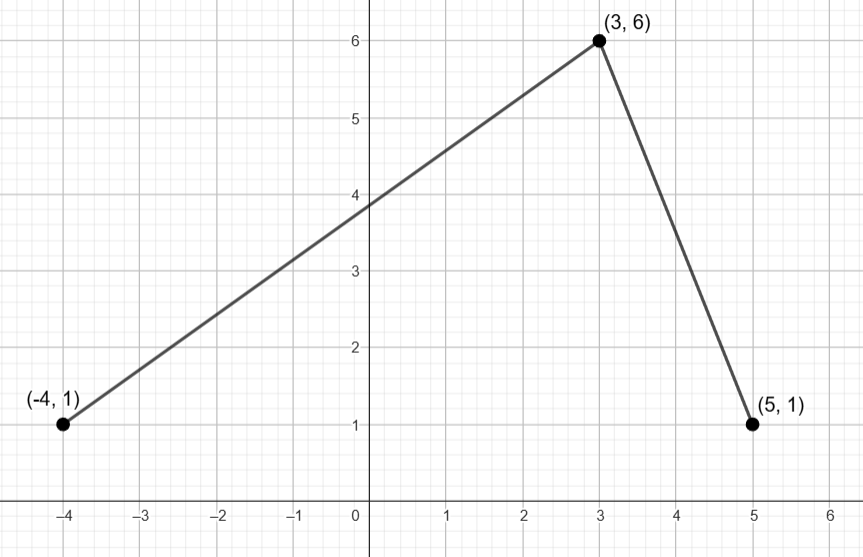
\includegraphics[width=10cm]{Opgave_21-30/Opgave_26/26.png}






\newpage
\subsection{Opgave 27}

En jernklods opvarmes og afkøles derefter af luften i lokalet. Afkølingen kan beskrives af funktionen

\begin{align*}
    a(t) = 20 + 880\cdot 0,95^t, t\geq 0
\end{align*}

hvor afkølingen påbegyndes til $t=0$ og $a(t)$ er klodsens temperatur målt i $^{\circ}C$ til tiden $t$, målt i minutter.

a) Tegn grafen for funktionen.

\ans
For at tegne grafen for funktionen kan vi opstille et sildeben for t værdierne 0, 3, 6, 9, 12.

\begin{tabular}{c|c|c|c|c|c}
    t & 0 & 3 & 6 & 9 & 12 \\\hline
    $a(t)$ & & & & &
\end{tabular}

Vi beregner nu $a(t)$ for de forskellige t værdier i sildebenet

\begin{align*}
    a(0) &= 20 + 880 \cdot 0.95^0 = 900.00 \\
    a(3) &= 20 + 880 \cdot 0.95^3 = 774.49 \\
    a(6) &= 20 + 880 \cdot 0.95^6 = 666.88 \\
    a(9) &= 20 + 880 \cdot 0.95^9 = 574.62 \\
    a(12) &= 20 + 880 \cdot 0.95^{12} = 495.52
\end{align*}

Udfylder vi sildebenet får vi

\begin{tabular}{c|c|c|c|c|c}
    t & 0 & 3 & 6 & 9 & 12 \\\hline
    $a(t)$ & 900 & 774,49 & 666,88 & 574,62 & 495,52
\end{tabular}

Nu kan vi så tage hver kolonne i sildebenet og indsætte dem som punkter i et koordinatsystem.
Den første kolonne svarer altså til punktet (0, 900) den næste kolonne til punktet (3, 774,49) osv.
Indsætter nu punkterne i et koordinatsystem og forbinder dem med en linje.
Den indtegnede funktion kan ses på billedet nedenfor.

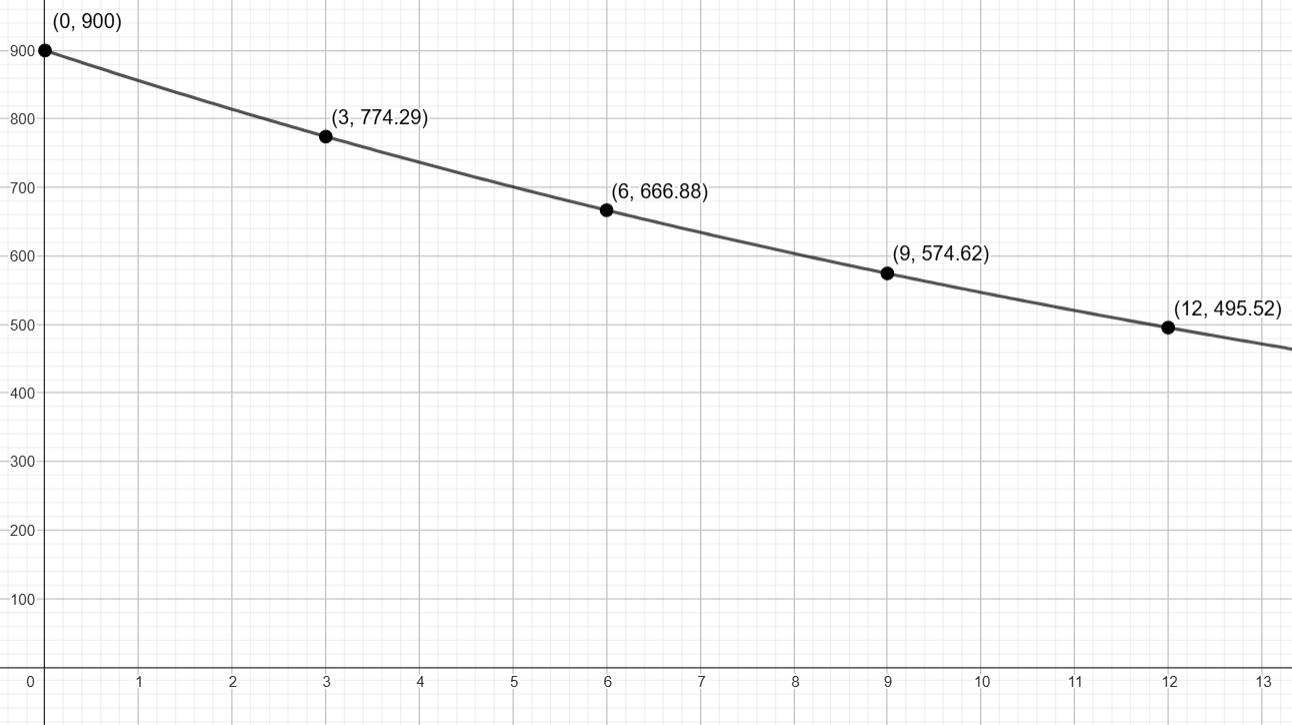
\includegraphics[width=10cm]{Opgave_21-30/Opgave_27/27.png}


b) Bestem $a(15)$

\ans
For at bestemme $a(15)$ bruger vi funktionen $a(t)$ og indsætter $t=15$. 
Vi beregner og får
\begin{align*}
    a(15) = 20 + 880\cdot 0,95^{15} = 427,70 
\end{align*}

Det betyder at efter $t = 15$ minutter er klodsens temperatur $a(15) = 427,70$ grader celcius. 


\newpage
\subsection{Opgave 28}

Funktionen f er bestemt ved

\begin{align*}
    f(x) = -2\cdot x + 4
\end{align*}

Forklar hvilken betydning tallene -2 og 4 har for grafens udseende.

\ans

Hvis vi sammenligner funktionen $f(x) = -2\cdot x + 4$
for forskellige funktioners forskrifter kan vi se at det er en lineær funktion 
da den matcher med den generelle forskrift for en lineær funktion
$f(x) = a\cdot x + b$.

Vi ved at a værdien for en lineær funktion er dens hældning, dvs når vi går en ud af x aksen, går funktionen hældningen
op eller ned. b værdien er funktionens skæring med y aksen.

Det vil sige at de -2 er hældningen for funktionen $f(x)$ og hver gang vi går 1 ud af x aksen
går funktionen 2 ned.

Tallet 4 fortæller at funktionen $f(x)$ skærer y aksen i $y = 4$.

Nedenfor er funktionen $f(x)$ indtegnet i GeoGebra hvor hældningen på -2 og skæringen med y aksen i 
$y = 4$ er markeret.

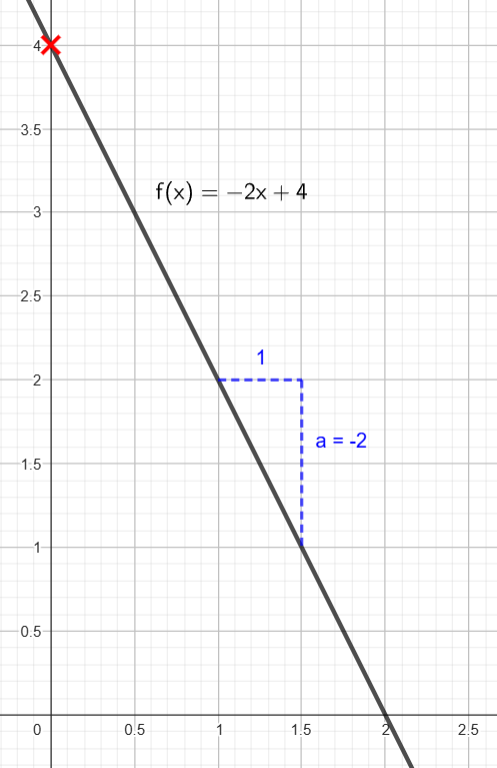
\includegraphics[width=6cm]{Opgave_21-30/Opgave_28/28.png}
\newpage
\subsection{Opgave 29}

For en elektrisk komponent er den afsatte effekt P proportional med strømstyrken I. Det oplyses, at
proportionalitetskonstanten er 12.

Opstil et udtryk for P som funktion af I.

\ans

Når vi opstillet et udtryk for P som funktion af I skrives dette som
$P(I)$. 

Vi får at vide at P er proportional med strømstyrken I, hvilket betyder at P er lig med I
ganget med en proportionalitetskonstant. Da proportionalitetskonstanten er 12 får vi altså udtrykket

\begin{align*}
    P(I) = 12\cdot I
\end{align*}
\newpage
\subsection{Opgave 30}

På figuren ses grafen for et andengradspolynomium på formen $f(x) = a\cdot x^2 +b\cdot x + c$.

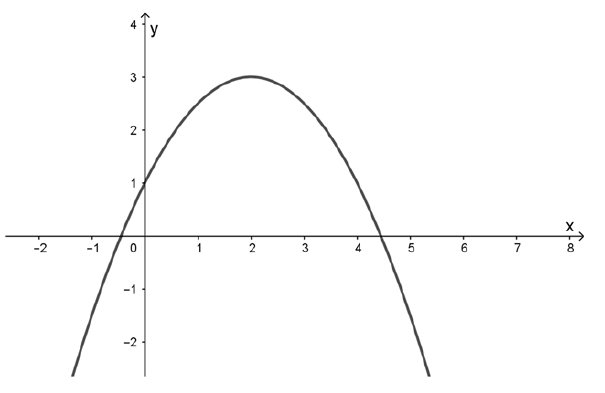
\includegraphics[width=8cm]{Opgave_21-30/Opgave_30/30.png}

Bestem fortegnet for a, og bestem fortegnet for c.

\ans

For et andengradspolynomium fortæller fortegnet af a om vores polynomie vender opad eller nedad.
Da andengradspolynomiet på figuren vender nedad er fortegnet for a dermed negativt.

For et andengradspolynomium er c værdien der hvor polynomiet skærer y aksen.
Da andengradspolynomiet på figuren skærer y aksen i $y = 1$ er fortegnet for c dermed positivt.





\newpage
\subsection{Opgave 31}

På figuren ses grafen for den lineære funktion f.

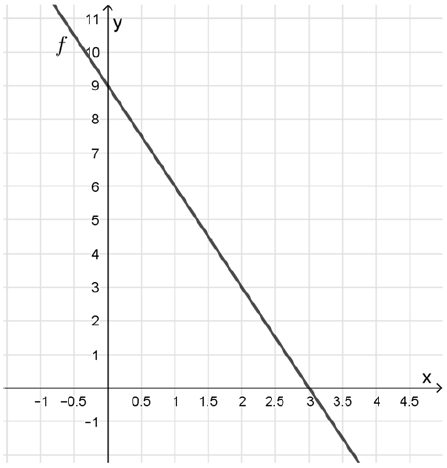
\includegraphics[width=8cm]{Opgave_31-40/Opgave_31/31.png}

a) Benyt figuren til at bestemme f(0)

\ans

For at finde $f(0)$ skal vi altså finde den y værdi vores funktion f har når 
vi står ved x værdien $x = 0$. Aflæser vi y værdien får vi at $f(0) = 9$.
Dette kan ses på figuren nedenfor

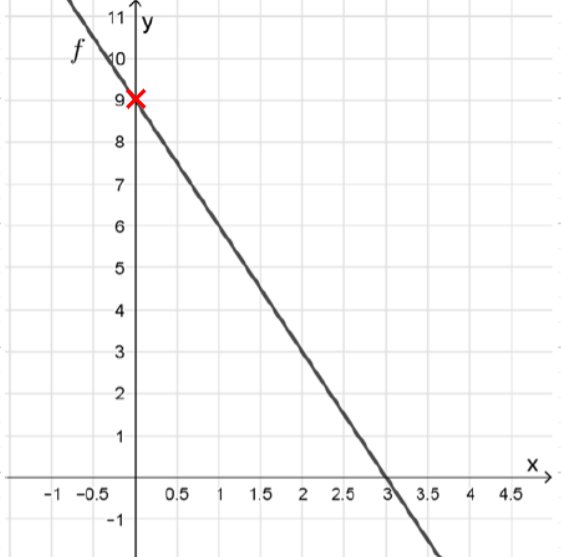
\includegraphics[width=8cm]{Opgave_31-40/Opgave_31/31.1.png}


b) Benyt figuren til at løse lignignen $f(x) = 0$

\ans

For at løse ligningen $f(x) = 0$ bliver vi bedt om at finde x værdien til funktionen f 
der hvor funktionen har y værdien 0 som er der hvor funktionen skærer x aksen.
Vi aflæser løsningen til $x = 3$.
Dette kan ses på figuren nedenfor

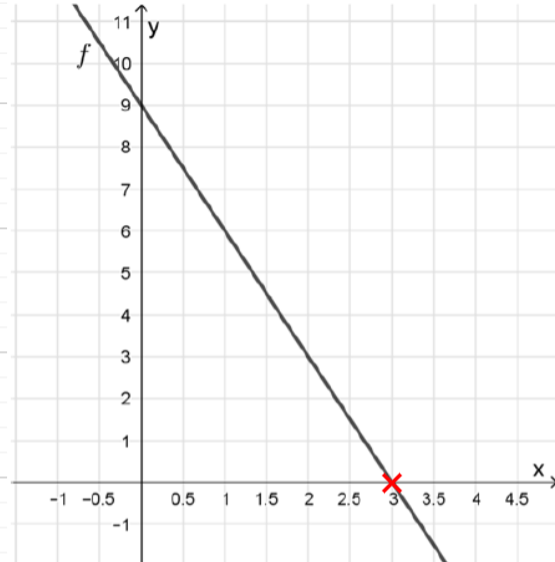
\includegraphics[width=8cm]{Opgave_31-40/Opgave_31/31.2.png}
\newpage
\subsection{Opgave 32}

På figuren ses graferne A, B og C for tre lineæra funktioner.

Det oplyses at funktionerne er bestemt ved forskrifterne

\begin{align*}
    f(x) &= 3x - 4\\
    g(x) &= 1,5x - 2\\
    h(x) &= 1,5x + 2
\end{align*}

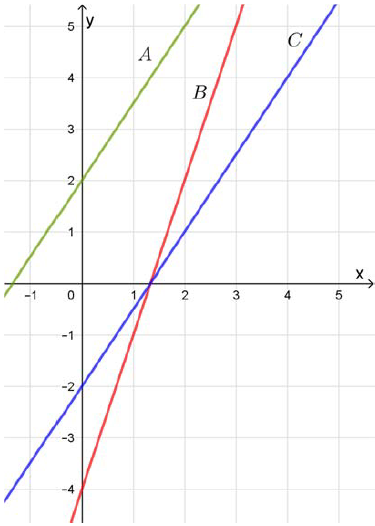
\includegraphics[width=8cm]{Opgave_31-40/Opgave_32/32.png}

Afgør hvilken graf der hører til hvilken funktion. Begrund svaret.

\ans

For en hver lineær funktion gælder det at dens b værdi er skæringen med y aksen.
Da en lineær funktion har den generelle forskrift $f(x) = ax + b$ kan vi altså se at b værdien for de
3 funktioner $f(x), g(x), h(x)$ har forskellige b værdier og dermed forskellige skæringer med y aksen.

Da $f(x)$ har b værdien $b = -4$ skærer den y aksen i $y = -4$ og svarer derfor til den røde lineære funktion B.

Da $g(x)$ har b værdien $b = -2$ skærer den y aksen i $y = -2$ og svarer derfor til den blå lineære funktion C.

Da $h(x)$ har b værdien $b = 2$ skærer den y aksen i $y = 2$ og svarer derfor til den grønne lineære funktion A.
\newpage
\subsection{Opgave 33}

Figuren viser grafen for et andengradspolynomium f.

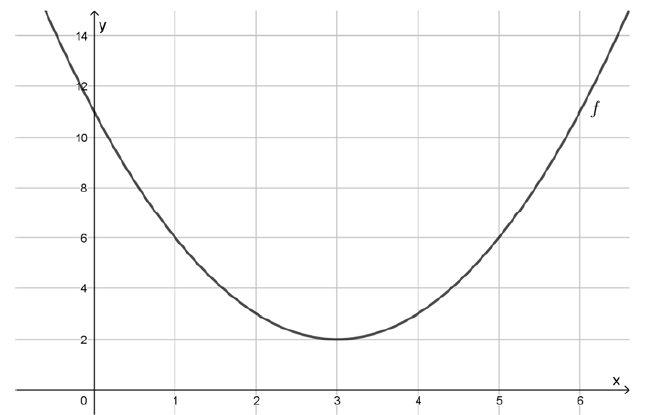
\includegraphics[width=8cm]{Opgave_31-40/Opgave_33/33.png}

Benyt grafen til at løse ligningen $f(x) = 6$

\ans

For at løse ligningen $f(x) = 6$ skal vi altså finde de steder funktionen har en y værdi på 6, og derefter aflæse de tilhørende x værdier.

Jeg tegner en vandret linje der går igennem $y = 6$ og aflæser x værdierne til de steder hvor den vandrette linje skærer funktionen f.

Jeg få de 2 x værdier og dermed de 2 løsninger $x = 1$ og $x = 5$.

Løsningerne er illustreret på nedenstående figur.

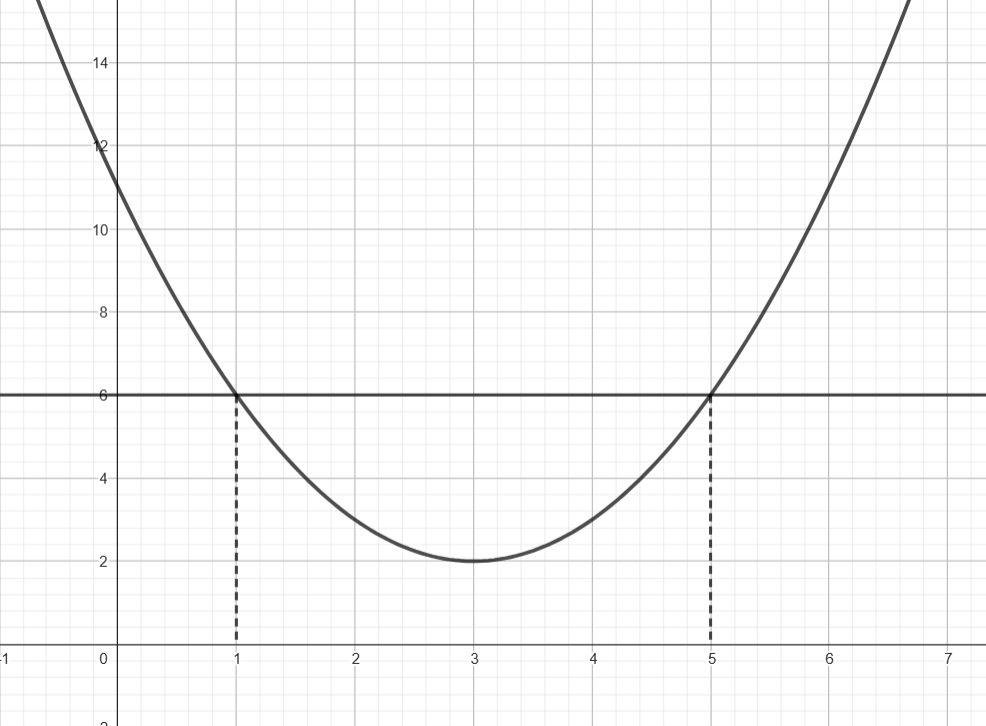
\includegraphics[width=8cm]{Opgave_31-40/Opgave_33/33.1.png}
\newpage
\subsection{Opgave 34}

Figuren viser graferne for to eksponentialfunktioner f og g bestemt ved

\begin{align*}
    f(x) = 0,5^x \\
    g(x) = 1,5^x
\end{align*}

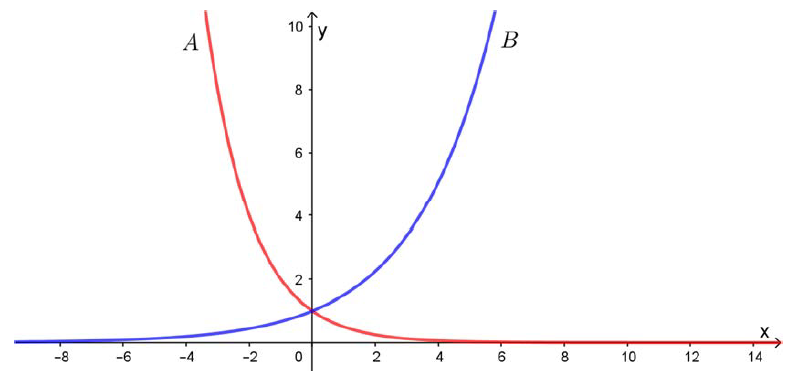
\includegraphics[width=8cm]{Opgave_31-40/Opgave_34/34.png}

Afgør hvilken graf, der hører til hvilken funktion.

\ans

Vi ved at eksponentialfunktioner har den generelle forskrift

$f(x) = a^x$

Vi ved yderligere at for en eksponentialfunktion gælder det at 

\begin{align*}
    &\text{funktionen er aftagende når} \hspace*{2mm} 0 < a < 1\\
    &\text{funktionen er voksende når} \hspace*{3mm} a > 1
\end{align*}

Da funktionen $f(x)$ har a værdien $a = 0,5$ ved vi at den er aftagende og derfor svarer til den røde funktion A som er aftagende.

Da funktionen $g(x)$ har a værdien $a = 1,5$ ved vi at den er voksende og derfor svarer til den blå funktion B som er voksende.

\newpage
\subsection{Opgave 35}

Figuren viser grafen for en eksponentialfunktion f.

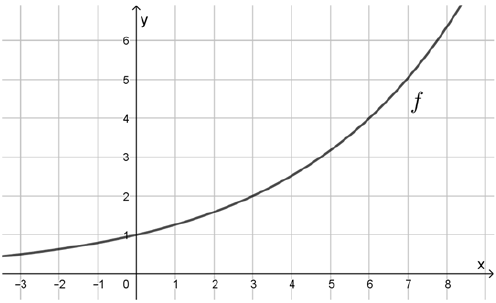
\includegraphics[width=8cm]{Opgave_31-40/Opgave_35/35.png}

Benyt figuren til at bestemme eksponentialfunktionens fordoblingskonstant.

\ans 

For at finde fordoblingskonstanten ud fra en graf skal vi gøre følgende.

Først vælger vi en værdi på y aksen. Jeg vælger $y  = 1$. S
Så går vi ud fra y aksen hvor $y = 1$ indtil vi rammer funktionen f, og aflæser den tilhørende x værdi.
Denne x værdi kalder vi for $x_1$ og aflæser værdien til $x_1 = 1$.

Nu fordobler vi den y værdi vi valgte til at starte med, og får den nye y værdi $y = 2$.
Vi går ud fra y aksen indtil vi rammer funktionen og aflæser den tilhørende x værdi.
Denne x værdi kalder vi for $x_2$ og aflæser værdien til $x_2 = 3$.

Nu kan vi beregne fordoblingskonstanten $T_2$ ved brug af formlen

\begin{align*}
    T_2 = x_2 - x_1
\end{align*}

Indsætter vi værdierne får vi

\begin{align*}
    T_2 = 3 - 1 = 2
\end{align*}

Fordoblingskonstanten for eksponentialfunktionen f er dermed 2.
På nedenstående figur kan man se hvordan de forskellige værdier er blevet aflæst.

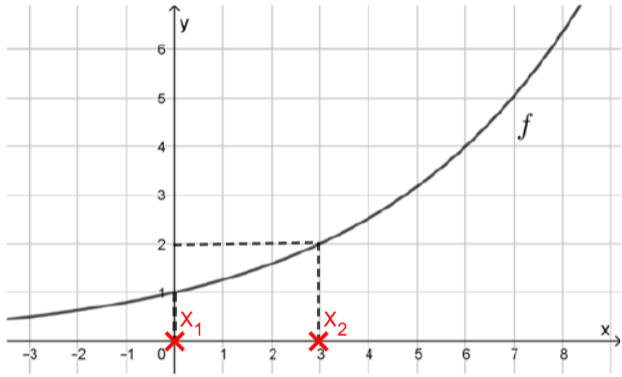
\includegraphics[width=8cm]{Opgave_31-40/Opgave_35/35.1.png}
\newpage
\subsection{Opgave 36}

På figuren ses graferne for tre andengradspolynomer f, g og h, som har forskrifterne

\begin{align*}
    f(x) &= -x^2 +2x +3\\
    g(x) &= -x^2 -2x + 1\\
    h(x) &= \frac{1}{4}x^2 -2x + 3
\end{align*}

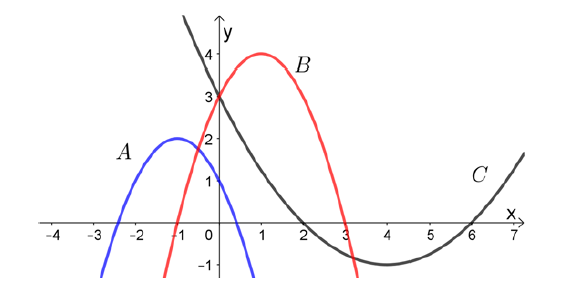
\includegraphics[width=8cm]{Opgave_31-40/Opgave_36/36.png}

Hvilken graf hører til hvilken funktion? Svaret skal begrundes.

\ans

Vi ved at der gælder følgende for en andengradspolynomium. 

Et andengradspolynomie har den generelle forskrift $ax^2 + bx + c$

Fortegnet for a værdien i et andengradspolynomium fortæller om grenene vender opad eller nedad.
Er a positivt $a > 0$ vender grenene opad.
Er a negativt $a < 0$ vender grenene nedad.

Værdien for c i et andengradspolynomium fortæller ved hvilken y værdi andengradspolynomiet skærer y aksen.

Ud fra disse informationer kan vi nu konkludere følgende.

Forskriften $g(x)$ har c værdien $c = 1$ hvilket betyder at $g(x)$ skærer y aksen i $y = 1$ og svarer derfor til det blå andengradspolynomium A
som er den eneste der skærer y aksen i $y = 1$.

Da begge forskrifter $f(x)$ og $h(x)$ skærer y aksen i samme værdi, kigger vi i stedet for på deres a værdier.

Forskriften $f(x)$ har en negativ a værdi $a = -1$ hvilet betyder at grenene på $f(x)$ vender nedad. $f(x)$ svarer derfor til det røde andengradspolynomium
B, hvis grene vender nedad.

Forskriften $h(x)$ har en positiv a værdi $a = \frac{1}{4}$ hvilket betyder at grenene på $h(x)$ vender opad. $h(x)$ svarer derfor til det sorte andengradspolynomium
C, hvis grene vender opad.  
\newpage
\subsection{Opgave 37}

Figuren viser graferne for en lineær funktion g og et andengradspolynomium f.

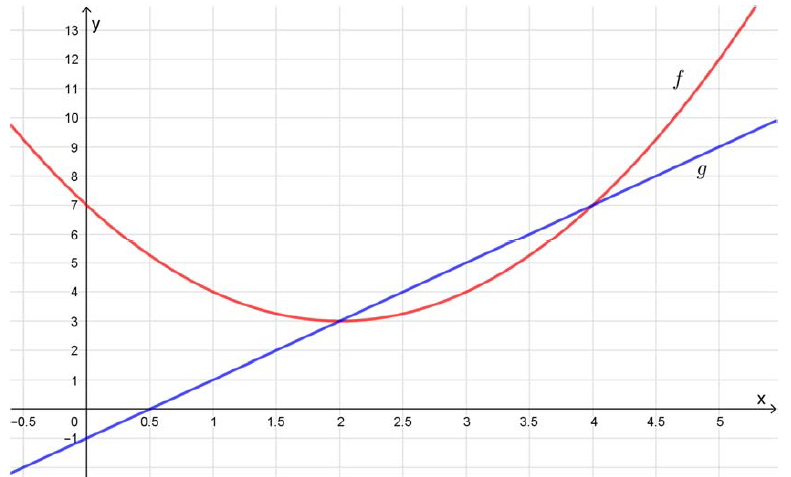
\includegraphics[width=8cm]{Opgave_31-40/Opgave_37/37.png}

Benyt figuren til at løse ligningen $g(x) = f(x)$.


\ans

For at løse ligningen $g(x) = f(x)$ skal vi altså finde de x værdier hvor y værdien for $g(x)$ og $f(x)$ er lig med hinanden.
Med andre ord skal vi finde x værdierne til de steder på grafen hvor $g(x)$ og $f(x)$ skærer hinanden.
Aflæser vi på grafen kan vi se at de skærer hinanden 2 steder ved x værdierne $x = 2$ og $x = 4$ hvilket er løsningen til ligningen $g(x) = f(x)$.
Skæringspunkterne er markerede på figuren nedenfor.

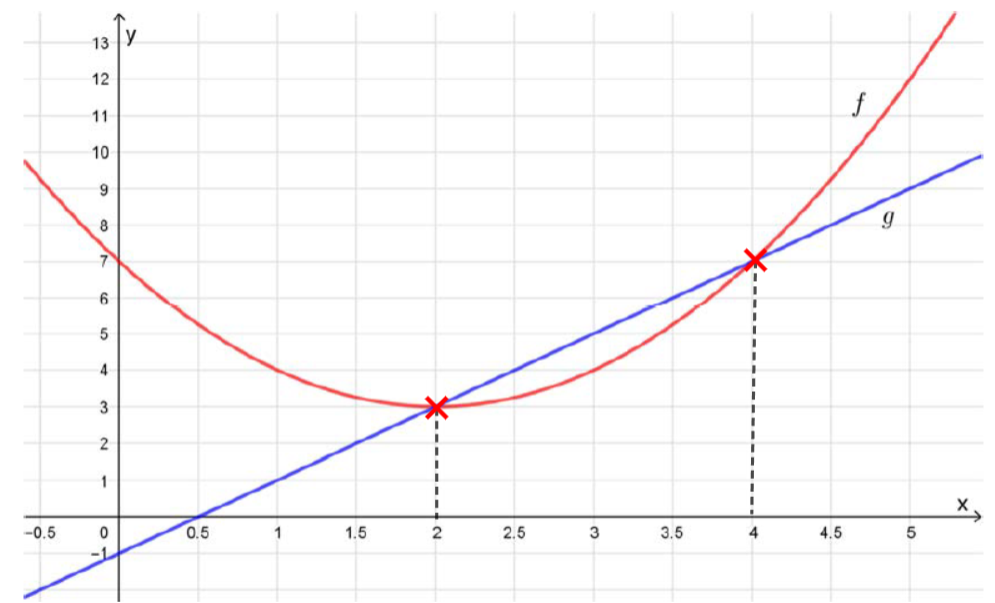
\includegraphics[width=8cm]{Opgave_31-40/Opgave_37/37.1.png}
\newpage
\subsection{Opgave 38}

Lad p være en funktion givet ved

\begin{align*}
    p(x) = 2x^4 -x^3 + 5x + 7
\end{align*}

Bestem skæringspunktet mellem grafen for p og koordinatsystemets y-akse.

\ans

For at finde skæringspunktet mellem funktionen p og koordinatsystemets y-akse kan vi udnytte at x værdien ved y aksen er $x = 0$.
Vi kan derefter bruge funktionen $p(x)$ og indsætte $x = 0$ for at beregne y værdien til der hvor $p(x)$ skærer y aksen.

\begin{align*}
    p(0) = 2\cdot 0^4 - 0^3 + 5 \dot 0 + 7 = 7
\end{align*}

Funktionen $p(x)$ skærer altså y aksen i $y = 7$. Da x værdien ved y aksen er $x = 0$ er skæringspunktet mellem funktionen $p(x)$ og koordinatsystemets y aksen dermed
$(0, 7)$.


\newpage
\subsection{Opgave 39}

Lad f betegne eksponentialfunktione givet ved $f(x) = 1,05^x$.

Bestem funktionens fordoblingskonstant.

\ans

For at finde fordoblingskonstanten, $T_2$ ud fra forskriften for en eksponentialfunktion kan vi bruge formlen

\begin{align*}
    T_2 = \frac{log(2)}{log(a)}
\end{align*}

Vi ved at den generelle forskrift for en eksponentialfunktion er $f(x) = a^x$ så i vores tilfælde er $a = 1,05$.
Indsætter vi værdierne i formlen får vi

\begin{align*}
    T_2 = \frac{log(2)}{log(1,05)} = 14.21
\end{align*}

Fordoblingskonstanten for eksponentialfunktionen $f(x)$ er dermed $T_2 = 14,21$


\newpage
\subsection{Opgave 40}

På en græsplæne måles hæjden af græsset lige efter en græsslåning til 45 millimeter. Gartneren ved, at græsset vokser 5 millimeter i døgnet.

Indfør passende variable, og opstil en model, som beskriver sammenhængen mellem græssets højde og tiden siden seneste slåning.

\ans

Da vi får at vide at græsset har en starthøjde og at det vokser med samme højde hvert døgn, ved vi at 
græsset følger en lineær model/funktion. Vi ved at den generelle forskrift for en lineær funktion er 
\begin{align*}
    f(x) = ax + b
\end{align*}

Værdien a fortæller hvor meget noget stiger med og værdien b fortæller os hvad startværdien er når $x = 0$.

Da vi har med tid at gøre, vælger jeg at udskifte x med t for antal døgn, og f med h for højde. 
Da græsset vosker med 5 millimeter i døgnet må vores a værdi være $a = 5$ og da græsset lige efter en græsslåning altså når $t = 0$ er 45 millimeter må vores b værdi være $b = 45$

Modellen som beskriver sammenhængen mellem græssets højde og antal døgn siden sidste slåning bliver derfor

\begin{align*}
    h(t) = 5t + 45
\end{align*}

Hvor $h(t)$ er højden i millimeter efter t døgn, t er antal døgn, 5 er antal millimeter græsset vosker med pr døgn og 45 er antal millimeter græsset er lige efter en græsslåning.
\newpage


\subsection{Opgave 41}

En gryde med vand varmes op på en kogeplade.

Lad t betegne tiden i minutter fra starten af målingerne og lad T betegne vandets temperatur. Til tiden 
$t=0$ er vandets temperatur $12^{circ}C$. Mens vandet opvarmes stiger temperaturen med $3^{\circ}C$ pr. minut.

Opstil en model for sammenhængen mellem vandes temperatur og tiden fra starten af målingerne.

\ans

Da vi får at vide at temperaturen stiger med den samme værdi for hvert minut og at vandet har en starttemperatur til tiden $t = 0$ 
har vi at gøre med en lineær model. Lineæra modeller eller lineære funktioner er på formen $f(x) = a\cdot x + b$ hvor a er hvor meget vores lineære model stiger eller falder pr x og 
b er vores startværdi der hvor $x = 0$. I vores tilfælde er $a = 3$, $b = 12$ og x er her t altså antallet minutter mens f er T altså temperaturen af vandet.
Vi får nu følgende model

\begin{align*}
    T(t) = 3\cdot t + 12
\end{align*}

$T(t)$ betegner altså vandets temperatur efter t minutter, 3 betegner antallet af grader vandet stiger med pr minut, t betegner antal minutter og 12 betegner 
vandets starttemperatur til tiden $t = 0$.



\newpage
\subsection{Opgave 42}

En lineær funktion f er bestemt ved 

\begin{align*}
    f(x) = -3\cdot x + 5
\end{align*}

Nogle værdier for f er vist i tabellen.

\begin{tabular}{|c|c|c|c|}
    \hline
    x & -1 & 0 & \\\hline
    $f(x)$ &  &  & 2 \\\hline 
\end{tabular}

Udfyld tabellens tomme felter.

\ans

For at udfylde felterne ud fra $f(x)$ indsætter vi de tilsvarende x værdier på x's plads i $f(x)$.

For den første kolonne har vi $x = -1$ og beregner $f(-1)$

\begin{align*}
    f(-1) = -3\cdot (-1) + 5 = 3 + 5 = 8
\end{align*}

For den anden kolonne har vi $x = 0$ og beregner $f(0)$

\begin{align*}
    f(0) = -3\dot 0 + 5 = 5
\end{align*}

I den diste kolonne kender vi kun værdien for $f(x)$ og vi skal så finde den tilsvarende værdi for x.

For at gøre dette skal vi altså løse ligningen $f(x) = 2$. Da vi ved at $f(x) = -3\cdot x + 5$ får vi

\begin{align*}
    -3\cdot x + 5 = 2 
\end{align*}

For at isolere x flytter vi først de 5 over på den anden side af lighedstegnet

\begin{align*}
    -3\cdot x + 5 - 5 = 2 - 5 \Leftrightarrow -3\cdot x = -3
\end{align*}

Nu dividerer vi med -3 på begge sider for at x kommer til at stå alene

\begin{align*}
    \frac{-3\cdot x}{-3} = \frac{-3}{-3} \Leftrightarrow x = 1
\end{align*}

Vi har nu alle værdierne for tabellens tomme felter, som er udfyldt nedenfor

\begin{tabular}{|c|c|c|c|}
    \hline
    x & -1 & 0 & 1 \\\hline
    $f(x)$ & 8 & 5 & 2 \\\hline 
\end{tabular}
\newpage
\subsection{Opgave 43}

En funktion f er bestemt ved 

\begin{align*}
    f(x) = 3\cdot x^2
\end{align*}

Nogle værdier for f er vist i tabellen.

\begin{tabular}{|c|c|c|c|}
    \hline
    x & -1 & 0 & 2 \\\hline
    $f(x)$ &  &  & \\\hline
\end{tabular}

Udfyld tabellens tomme felter.

\ans

For at udfylde tabellens tomme felter skal vi for hver kolonnes x værdi beregne den tilsvarende værdi for $f(x)$ ved at indsætte x værdien i forskriften 
$f(x) = 3\cdot x^2$

For den første kolonne og x værdien $x = -1$ får vi den tilsvarende værdi

\begin{align*}
    f(-1) = 3\cdot (-1)^2 = 3 \cdot 1 = 3
\end{align*}

For den anden kolonne og x værdien $x = 0$ får vi den tilsvarende værdi

\begin{align*}
    f(0) = 3\cdot 0^2 = 3 \cdot 0 = 0
\end{align*}

For den første kolonne og x værdien $x = 2$ får vi den tilsvarende værdi

\begin{align*}
    f(2) = 3\cdot 2^2 = 3 \cdot 4 = 12
\end{align*}

Den udfyldte tabel kan ses nedenfor

\begin{tabular}{|c|c|c|c|}
    \hline
    x & -1 & 0 & 2 \\\hline
    $f(x)$ & 3 & 0 & 12 \\\hline
\end{tabular}


\newpage
\subsection{Opgave 44}

Grafen for en funktion f er vist på nedenstående figur.

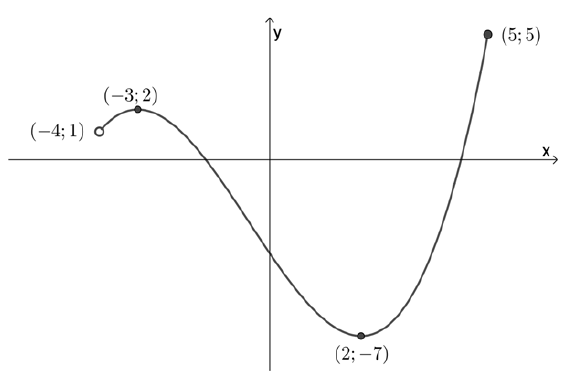
\includegraphics[width=8cm]{Opgave_41-50/Opgave_44/44.png}

Angiv funktionens monotoniforhold.

\ans

Når vi angiver en funktions monotoniforhold skal vi angive i hvilke intervaller vores funktion er voksende
og i hvilke intervaller vores funktion er aftagende.

Starter vi fra de laveste x værdier på vores funktion kan vi se at den er voksende mellem det åbne punkt $(-4; 1)$ og det lukkede punkt $(-3; 2)$ så f er voksende i intervallet
$\rbrack -4; -3 \rbrack$.

Fra det lukkede punkt $(-3; 2)$ til det lukkede punkt $(2; -7)$ er f aftagende så f er aftagende i intervallet
$[-3; 2]$.

Fra det lukkede punkt $(2; -7)$ til det lukkede punkt $(5; 5)$ er f voksende så f er voksende i intervallet $[2; 5]$.

Funktionen f har altså følgende monotoniforhold

Voksende i intervallerne: $\rbrack -4; -3\rbrack$, $[2; 5]$

Aftagende i intervallerne: $[-3; 2]$
\newpage
\subsection{Opgave 45}

Tabellen viser antal frøer N i et vandhul i perioden fra 2012-2015. Tiden t måles i år fra 2012.

Følgende data er tilgængelige:

\begin{tabular}{|c|c|c|c|c|}
    \hline
    Tid t & 0 & 1 & 2 & 3 \\\hline
    Antal frøer N & 4520 & 4260 & 4000 & 3750
\end{tabular}

Det oplyses, at udviklingen i antal frøer tilnærmelsesvis kan beskrives ved en model på formen:

\begin{align*}
    N(t) = a\cdot t + b
\end{align*}

a) Bestem a og b.

\ans

Da vi får at vide at udviklingen i antal frøer kan beskrives ved $N(t) = a\cdot t + b$ ved vi at udviklingen beskrives ved en lineær model $f(x) = a\cdot x + b$

Ud fra 2 datapunkter kan vi altså beregne a værdien ved formlen

\begin{align*}
    a = \frac{y_2 - y_1}{x_2 - x_1}
\end{align*}

Jeg vælger den første kolonne (0, 4520) og den sidste kolonne (3, 3750) som mine 2 datapunkter så jeg får
$(x_1, y_1) = (0, 4520)$ og $(x_2, y_2) = (3, 3750)$. Beregner nu a værdien

\begin{align*}
    a = \frac{3750 - 4520}{3 - 0} = \frac{-770}{3} = -256,67
\end{align*}

For en lineær funktion kan vi beregne b værdien ved følgende formel

\begin{align*}
    b = y_1 - a \cdot x_1
\end{align*}

Indsætter vi tallene får vi

\begin{align*}
    b = 4520 - (-256,67) \cdot 0 = 4520
\end{align*}

Vi har nu værdierne $a = -256,67$ og $b = 4520$.

b) Hvad fortæller tallet a om udviklingen i antal frøer?

\ans

Tallet a fortæller om hvor meget antallet af frøer ændrer sig for hvert år t.
Da a værdien er $a = -256,67$ betyder det altså at antallet af frøer i vandhullet falder med ca 256 frøer om året.

\newpage
\subsection{Opgave 46}

Intensiteten af strålingen fra en mobiltelefon aftager, når afstanden til mobiltelefonen øges. I tabellen ses sammenhørende værdier af intensitet I og afstand x. Der ses bort fra enheder.

\begin{tabular}{|c|c|c|c|c|c|}
    \hline
    Afstand $x$ & 0,01 & 0,05 & 0,1 & 0,2 & 1 \\\hline
    Intensitet $I$ & 201,00 & 9,20 & 2,02 & 0,45 & 0,02 \\\hline
\end{tabular}

Det vides, at intensiteten I og afstenden x tilnærmelsesvist kan beskrives med en model på formen 

\begin{align*}
    I(x)=b\cdot x^a
\end{align*}

Bestem a og b.

\ans

Når vi har en model på formen $f(x) = b\cdot x^a$ har vi at gøre med en potens funktion.

For en potens funktion kan vi beregne a værdien ud fra 2 datapunkter $(x_1, y_1)$ og $(x_2, y_2)$ ved følgende formel

\begin{align*}
    a = \frac{log(y_2) - log(y_1)}{log(x_2) - log(x_1)}
\end{align*}

Jeg vælger den første kolonne som mit første datapunkt og den sidste kolonne som mit andet datapunkt og får
$(x_1, y_1) = (0,01, 201,00)$ og $(x_2, y_2) = (1, 0,02)$.

Indsætter værdierne og får

\begin{align*}
    a = \frac{log(0,02) - log(201,00)}{log(1) - log(0,01)} = -2,00 
\end{align*}

For at bestemme b værdien bruger vi formlen 

\begin{align*}
    b = \frac{y_1}{x_1^a}
\end{align*}

Indsætter vi værdierne får vi

\begin{align*}
    b = \frac{201,00}{0,01^{-2,00}} = 0,0201
\end{align*}

Vi får altså værdierne $a = -2,00$ og $b = 0,0201$
\newpage
\subsection{Opgave 47}

Funktionen f er bestemt ved forskriften 

\begin{align*}
    f(x) = 4x^3 + 5x^2 + 8
\end{align*}

Bestem f'(2).

\ans

For at bestemme f'(2) skal vi først bestemme f'(x).

Når vi bestemmer f'(x) betyder det at vi differentierer f(x).

Der gælder følgende 

\begin{align*}
    f(x) &= a\cdot x^n\\
    f'(x) &= n\cdot a \cdot x^{n-1}
\end{align*}

Når vi differentierer en konstant, a ganget på x $a\cdot x$ får vi konstanten a.

Når vi differentierer konstanter (tal) så bliver de altid 0.
I vores tilfælde består $f(x)$ af flere led så vi kan anvende de ovenstående regler på alle ledene. Vi får

\begin{align*}
    f'(x) = 3\cdot 4x^{3-1} + 2\cdot 5x^{2-1} + 0 = 12x^2 + 10x
\end{align*}

Nu har vi beregnet f'(x), og for at bestemme f'(2) indsætter vi bare 2 på x's plads i f'(x). Vi får

\begin{align*}
    f'(2) = 12\cdot 2^2 + 10\cdot 2 = 12\cdot 4 + 20 = 68
\end{align*}

Vi får altså svaret $f'(2) = 68$
\newpage
\subsection{Opgave 48}

Funktionen f er bestemt ved forskriften 

\begin{align*}
    f(x) = 3x^2 + 4x - 1
\end{align*}

Bestem en ligning for tangenten til grafen for f i punktet (1; 6).

\ans

For at bestemme ligningen for tangenten til en graf i et punkt skal vi bruge følgende formel

\begin{align*}
    y = f(x_0) + f'(x_0)\cdot (x - x_0)
\end{align*}

Her er $x_0$ x værdien til punket, $f(x_0)$ er y værdien til punktet og $f'(x_0)$ er hældningen af $f(x)$ i x værdien $x_0$.

Fra punktet ved vi at $x_0 = 1$ og $f(x_0) = 6$. Vi bestemmer nu $f'(x)$ ligesom i opgave 47.

\begin{align*}
    f'(x) = 2 \cdot 3x^{2-1} + 4 - 0 = 6x + 4
\end{align*}

Vi kan nu bestemme $f'(x_0) = f'(1)$ ved at indsætte 1 på x's plads i $f'(x)$

\begin{align*}
    f'(1) = 6\cdot 1 + 4 = 10
\end{align*}

Indsætter vi nu alle værdierne i formlen for tangentens ligning får vi

\begin{align*}
    y = 6 + 10\cdot (x - 1) = 6 + 10\cdot x - 10 = 10x - 4
\end{align*}

Tangentens ligning til $f(x)$ i punktet (1; 6) er derfor

\begin{align*}
    y = 10x - 4
\end{align*}
\newpage
\subsection{Opgave 49}

På figuren ses grafen for funktionen f.

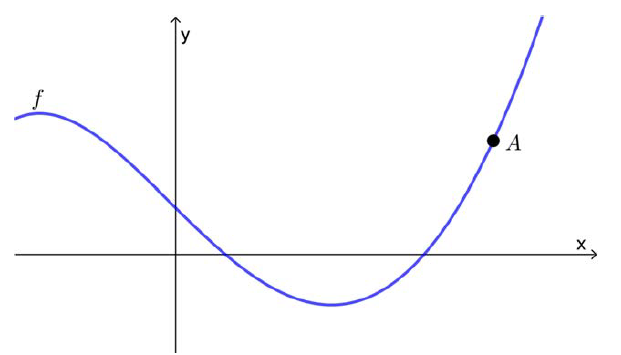
\includegraphics[width=8cm]{Opgave_41-50/Opgave_49/49.png}

Tegn både en sekant og en tangent gennem punkt A.

\ans

En tangent igennem et punkt er en ret linje som går igennem punktet og følger hældningen på funktionen i punket.

En sekant igennem et punkt er en ret linje som går igennem punktet og 1 andet vilkårligt punkt på grafen.

Nedenfor er tangenten indtegnet som den røde linje og sekanten indtegner som den sorte linje.

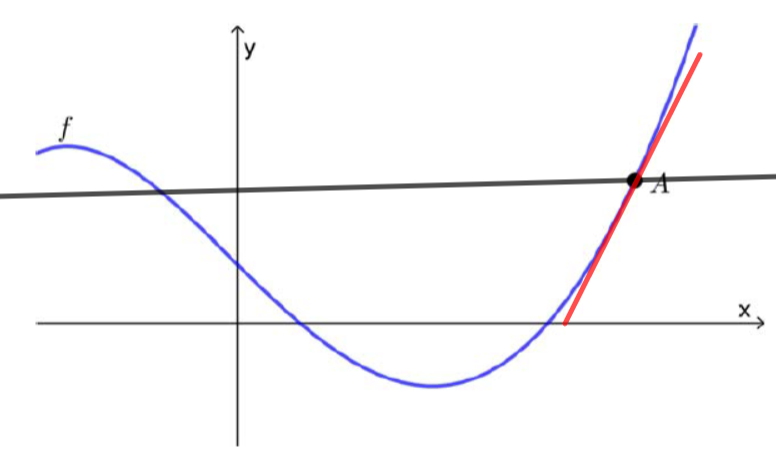
\includegraphics[width=8cm]{Opgave_41-50/Opgave_49/49.1.png}


\newpage
\subsection{Opgave 50}

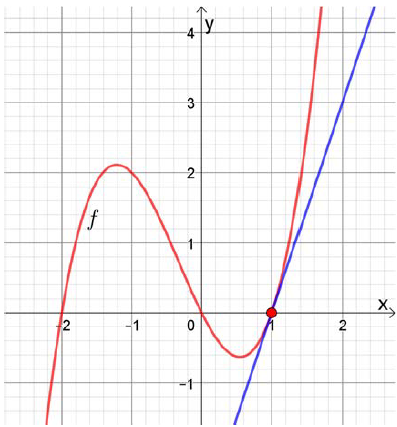
\includegraphics[width=8cm]{Opgave_41-50/Opgave_50/50.png}

Figuren viser grafen for en funktion f og dens tagnet i $x = 1$.

Benyt figuren til at bestemme $f'(1)$.

\ans

For at bestemme $f'(1)$ skal vi altså bestemme hældningen for $f(x)$ i det punkt hvor $x = 1$. Da vi også er givet tangenten til 
$f(x)$ i $x = 1$ og da hældningen på tangenten i $x = 1$ og $f'(1)$ er det samme kan vi altså aflæse tangentens hældning.

Da tangenten er en ret linje, kan vi aflæse den hældning ved at gå 1 hen ad x aksen, og så op af y aksen indtil vi rammer tangenten igen.
Det stykke vi bevæger os op vil så svare til tangentens hældning og dermed $f'(1)$. Går vi en hen ad x aksen skal vi bevægge os 3 op ad y aksen
før vi rammer tangenten igen. Hældningen på tangenten er dermed 3 og derfor er $f'(1) = 3$. Figuren nedenfor viser aflæsningen af tangentens hældning.

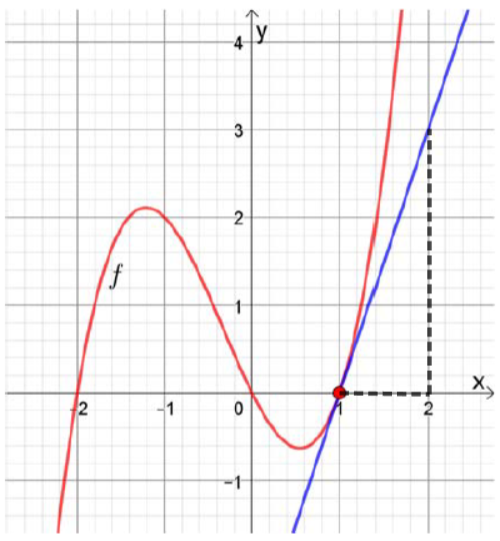
\includegraphics[width=8cm]{Opgave_41-50/Opgave_50/50.1.png}
\newpage


\subsection{Opgave 51}

Nedenfor ses grafen for en funktion f.

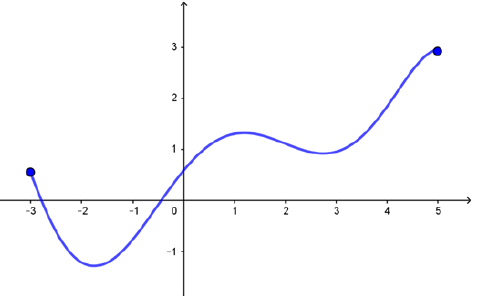
\includegraphics[width=8cm]{Opgave_51-56/Opgave_51/51.png}

Benyt grafen til at bestemme fortegnet på $f'(-1)$.

\ans

Har vi en graf $f(x)$ så fortæller fortegnet på $f'(x)$ i en bestemt x værdi om vores funktion $f(x)$
har en positiv hældning, altså at den er voksende eller at den har en negativ hældning, altså at den er aftagende.

Kigger vi på grafen hvor $x = -1$ kan vi se at $f(x)$ er voksende hvilket betyder at fortegnet for $f'(-1)$ er positivt.




\newpage
\subsection{Opgave 52}

Grafen for en funktion f er vist på nedenstående figur.

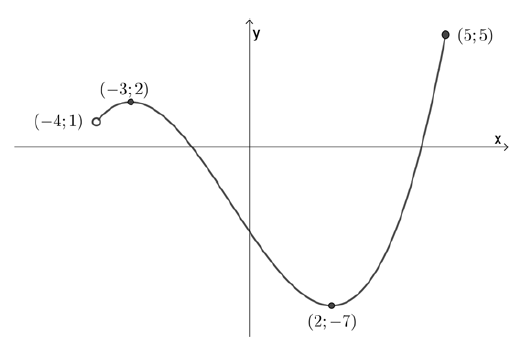
\includegraphics[width=8cm]{Opgave_51-56/Opgave_52/52.png}

Løs ligningen $f'(x) = 0$.

\ans

Når vi bliver bedt om at løse ligningen $f'(x) = 0$ bliver vi bedt om at finde de x værdier hvor hældningen på 
$f(x)$ er lig med 0. I de x værdier hvor hældningen for $f(x)$ er lig med 0 er de x værdier hvor tangenten i x værdien ville ligge horizontalt.
Dette sker typisk ved en funktions maksimums eller minimums punkter. I vores tilfælde kan vi se 2 x værdier hvor tangenten i de x værdier ville være horizontale.
Dette er tilfældet ved x værdierne $x = -3$ og $x = 2$. Det betyder at løsningen til ligningen $f'(x) = 0$ er 
$x = -3$ og $x = 2$. Tangenterne i de x værdier kan ses på figuren nedenfor  

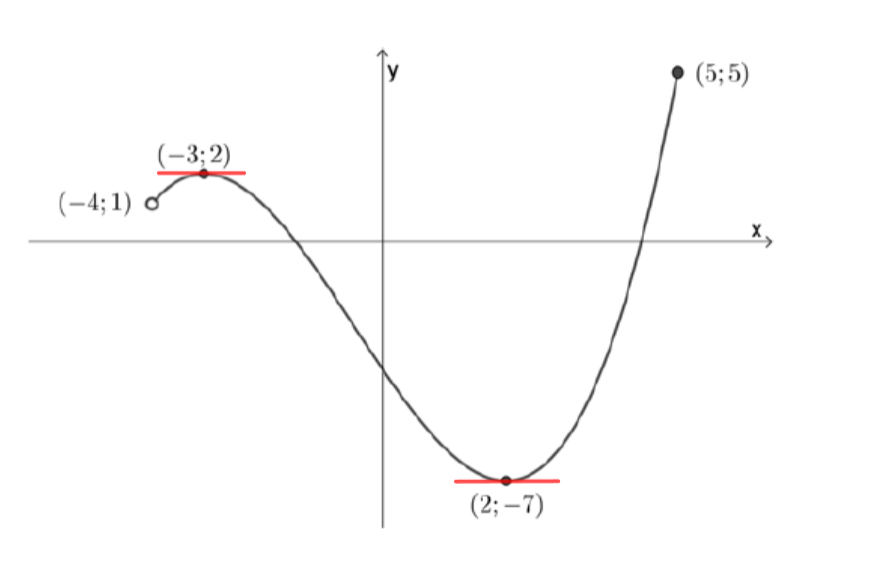
\includegraphics[width=8cm]{Opgave_51-56/Opgave_52/52.1.png}
\newpage



\end{document}